\section{Description of the server}
\label{sec:Description of the server}

We implemented our server in Java. Our server receives request and if it is busy proccessing one,
coming request will be added to the queue and proccessed later. The server can be either
single threaded (SimpleServer.java) meaning that it can only process one request at a time. Or
it can use multiple thread(ThreadedServer.java) to process several requests at the same time.

\subsection{Computation performed by the server}
\label{sub:Computation performed by the server}
The compution performed by the server consist of calculating the power of a
two-dimensional Matrix $M$ powered by a natural $p$.

\subsection{Request and response format}
\label{sub:Request and response format}

Each client request contains the matrix and the exposant. To achieve the
measurement that were asked, we added some fields to the request to get
some information such as computation time and and response time. We also
give an identifier to a request to make a mapping between request and response.

\section{Description of the measurement setup}
\label{sec:Description of the measurement setup}

\subsection{Used hardwares and softwares}
\label{sub:Used hardwares and softwares}

For our tests, two computer from the Intel room were used (in the Reaumur
building), they have the following specifications :

\begin{tabular}{|l|l|}
    \hline
    Processor & Intel(R) Core(TM)2 Quad Q6600 \@ 2.40GHz \\
    Instruction set & 64-bit \\
    \hline
    Total memory & 3981192 kB \\
    Total swap & 4063228 kB \\
    \hline
    Ethernet controller & Intel Corporation 82566DM-2 Gigabit Network Connection \\
    \hline
\end{tabular}
\bigskip

Those computers run on Linux (centOS distribution) so we used \enquote{top},
\enquote{htop} and \enquote{grep} to monitor CPU load and \enquote{Wireshark}
to monitor network usage (because nor \enquote{NetHogs} nor \enquote{iftop} were
installed). \newline

\subsection{Description of the load generator}
\label{sub:Description of the load generator}
We implemented a LoadGenerator to simulate the behavior of many independent
clients. The LoadGenerator uses the inversion method to generate exponentiallly
distributed randoms numbers to create inter-request times.

\section{Measurements and modeling}
\label{sec:Measurements and modeling}

\subsection{Measurement of individual client requests}
\label{sub:Measurement of individual client requests}

The figure~\ref{fig:measurement1} shows the evolution of the average time needed
according to size-changing matrices. For the lower sized matrices, the network
time is the most impactful factor on the average time because the server needs a negligible time
to process the matrix. Furthermore, the request contained much more information than the matrix
(because we used timestamp and other information) so the ratio between the total size of the request
and the ''real content'' size (size of the matrix) is low at beginning and increases as the matrix grows.

\begin{figure}[!ht]
    \centering
    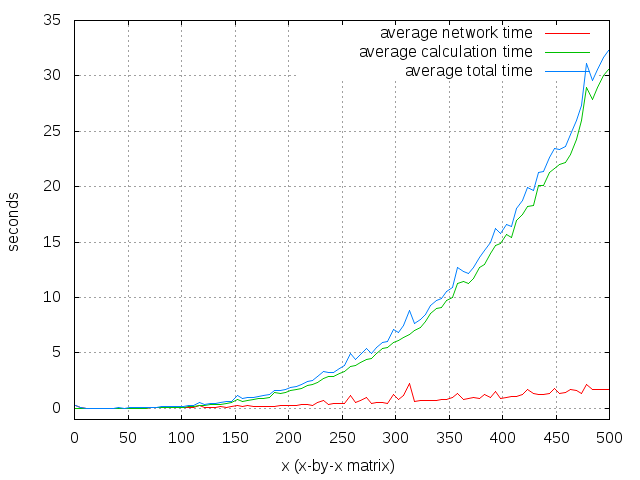
\includegraphics[width=0.5\linewidth]{measurement1.png}
    \caption{Measurement of average time needed depending on size-changing matrices}
    \label{fig:measurement1}
\end{figure}

\subsection{Measurement of the load generator}
\label{sub:Measurement of the load generator}

The figure~\ref{fig:histocpu} shows the average CPU load for different request rate. As one could
expect, when the request rate increases the average CPU load increases too. One thing important
on this figure concerns the CPU load for request rate superior to 0.5. Indeed, we can see that the 
CPU load exceeds the 100\%\footnote{the top command express CPU load on one CPU even if multiple
CPU are runnning}. This suggest that when the arrival rate exceeds 0.5, the server has an hard time
processing the incoming request. 

\begin{figure}[!ht]
    \centering
    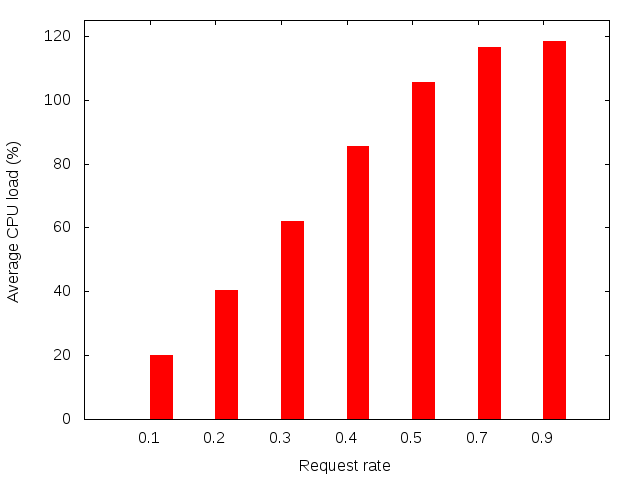
\includegraphics[width=0.5\linewidth]{cpu_load.png}
    \caption{Histogram of the CPU load for multiple arrival rates}
    \label{fig:histocpu}
\end{figure}
The figure~\ref{fig:histonetwork} shows the network load for different request rate. We can see that
network load does not differ much. This happens simply because we have done our measuremnt with the 
LoadGenerator sending 500 requests of variying size with different request rate so it's understandable to have the network load around 290 MB for each rate
\begin{figure}[!ht]
    \centering
    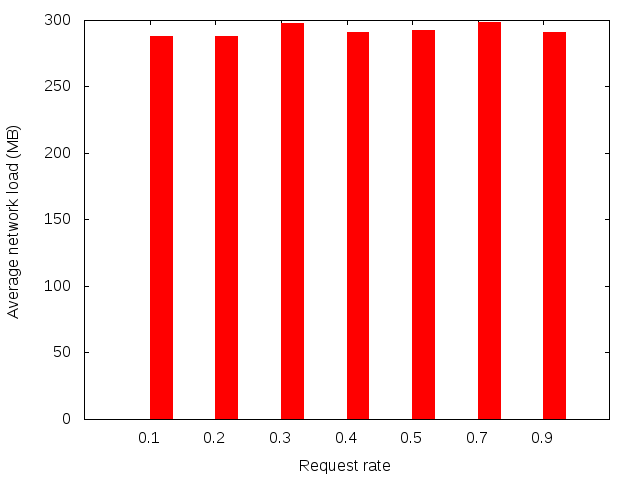
\includegraphics[width=0.5\linewidth]{network_load.png}
    \caption{Histogram of the network load for multiple arrival rates}
    \label{fig:histonetwork}
\end{figure}

The figure~\ref{fig:historesponse} shows the average response time for several arrival rates.
We can notice on this figure, that the average response time skyrockets between arrival rate 
0.5 and arrival rate 0.7 . The reason of this phenomenon is explained in the following section but 
it's the average waiting time that has a most impact on the response time. Request arrives too fast 
for the server, so they keep being accumulating in the queuing making them wait for a longer period
of time. 
\begin{figure}[!ht]
    \centering
    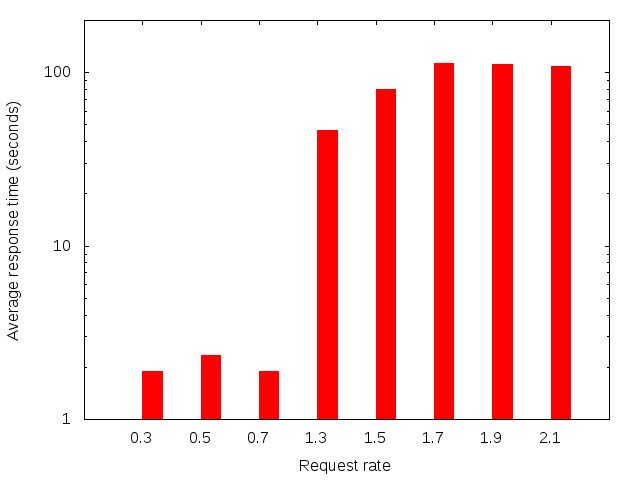
\includegraphics[width=0.5\linewidth]{responsetime.png}
    \caption{Histogram of the response time for multiple arrival rates}
    \label{fig:historesponse}
\end{figure}

\subsection{Queueing station model}
\label{sub:Queueing station model}
For our queueing station model, we used an \texttt{M/M/1} queue. For each
arrival rate($\lambda$) and service rate($\mu$), we computed the
average response time and the average waiting time in the queue. Notice that
every value expressed in the tables below are in second.

$\lambda$ = 0.1 , $\mu$ = 0.65:
\begin{minipage}{\linewidth}
    \bigskip
    \begin{minipage}{0.45\linewidth}
        \begin{tabular}{|l|l|}
            \hline
            Theory & \\
            \hline
            Average time spent in system & 1.8182 \\
            Average waiting time & 0.2797 \\
            \hline
        \end{tabular}
    \end{minipage}
    \begin{minipage}{0.45\linewidth}
        \begin{tabular}{|l|l|}
            \hline
            Experimental & \\
            \hline
            Calculation time & 765.78 \\
            Average calculation time & 1.53 \\
            Queue time & 115.282 \\
            Average waiting time & 0.23 \\
            Average time spent in system & 1.76 \\
            \hline
        \end{tabular}
    \end{minipage}
    \bigskip
\end{minipage}

\begin{minipage}{\linewidth}
    $\lambda$ = 0.2, $\mu$ = 0.66:

    \bigskip
    \begin{minipage}{0.45\linewidth}
        \begin{tabular}{|l|l|}
            \hline
            Theory & \\
            \hline
            Average time spent in system & 2.2222 \\
            Average waiting time & 0.6838 \\
            \hline
        \end{tabular}
    \end{minipage}
    \begin{minipage}{0.45\linewidth}
        \begin{tabular}{|l|l|}
            \hline
            Experimental & \\
            \hline
            Calculation time & 758.96718 \\
            Average calculation time & 1.517934 \\
            Queue time & 344.924 \\
            Average waiting time & 0.6898 \\
            Average time spent in system & 2.20778 \\
            \hline
        \end{tabular}
    \end{minipage}
    \bigskip
\end{minipage}

\begin{minipage}{\linewidth}
    $\lambda$ = 0.3, $\mu$ = 0.646 :

    \bigskip
    \begin{minipage}{0.45\linewidth}
        \begin{tabular}{|l|l|}
            \hline
            Theory & \\
            \hline
            Average time spent in system & 2.9412 \\
            Average waiting time & 1.3787 \\
            \hline
        \end{tabular}
    \end{minipage}
    \begin{minipage}{0.45\linewidth}
        \begin{tabular}{|l|l|}
            \hline
            Experimental & \\
            \hline
            Calculation time & 772.9727 \\
            Average calculation time & 1.545945 \\
            Queue time & 707.31 \\
            Average waiting time & 1.41462 \\
            Average time spent in system & 2.9605 \\
            \hline
        \end{tabular}
    \bigskip
    \end{minipage}
\end{minipage}

\begin{minipage}{\linewidth}
    $\lambda$ =0.4, $\mu$ = 0.687 :

    \bigskip
    \begin{minipage}{0.45\linewidth}
        \begin{tabular}{|l|l|}
            \hline
            Theory & \\
            \hline
            Average time spent in system & 3.4843 \\
            Average waiting time & 2.0287 \\
            \hline
        \end{tabular}
    \end{minipage}
    \begin{minipage}{0.45\linewidth}
        \begin{tabular}{|l|l|}
            \hline
            Experimental & \\
            \hline
            Calculation time & 727.67711 \\
            Average calculation time & 1.4553542 \\
            Queue time & 1214.914 \\
            Average waiting time & 2.429828 \\
            Average time spent in system & 3.8851 \\
            \hline
        \end{tabular}
    \end{minipage}
    \bigskip
\end{minipage}

\begin{minipage}{\linewidth}
   $\lambda$=0.5 , $\mu$ = 0.7045:

    \bigskip
    \begin{minipage}{0.45\linewidth}
        \begin{tabular}{|l|l|}
            \hline
            Theory & \\
            \hline
            Average time spent in system & 4.902 \\
            Average waiting time & 3.4815 \\
            \hline
        \end{tabular}
    \end{minipage}
    \begin{minipage}{0.45\linewidth}
        \begin{tabular}{|l|l|}
            \hline
            Experimental & \\
            \hline
            Calculation time & 709.71048 \\
            Average calculation time & 1.4194 \\
            Queue time & 3427.032 \\
            Average waiting time & 6.854064 \\
            Average time spent in system & 8,273464 \\
            \hline
        \end{tabular}
    \end{minipage}
    \bigskip
\end{minipage}

\begin{minipage}{\linewidth}
   $\lambda$=0.7, $\mu$ = 0.6763:

    \bigskip
    \begin{minipage}{0.45\linewidth}
        \begin{tabular}{|l|l|}
            \hline
            Theory & \\
            \hline
            Average time spent in system & N/A \\
            Average waiting time & N/A \\
            \hline
        \end{tabular}
    \end{minipage}
    \begin{minipage}{0.45\linewidth}
        \begin{tabular}{|l|l|}
            \hline
            Experimental & \\
            \hline
            Calculation time & 739.24599 \\
            Average calculation time & 1.478491 \\
            Queue time & 58704.59 \\
            Average waiting time & 11,740918 \\
            Average time spent in system & 13,219409 \\
            \hline
        \end{tabular}
    \end{minipage}
    \bigskip
\end{minipage}

As we can see, the model performs quite well for $\lambda$ <0.5 . For example, with $\lambda$ = 0.3,
we obtained an average time spent in the system of 2.9412 second with while the measured value gives us
2.9605 which is not so far from the value given by the model. When the $\lambda$ value equals 0.5, the
model does not fit anymore. The average waiting time measured far surpasses the model (almost the
double). This be can explained, by the fact that the $\lambda$ get closer to the $\mu$ such that more
request arrives in the queue than the one that leave the queue. This lead to a growing queue so request 
arriving must wait longer.


\subsection{Improvement of the performance of the system}
\label{sub:Improvement of the performance of the system}
The improvement we choose to do is the usage of job priorities. Instead of using a FCFS queue, 
the server uses a priority queue. The queue is sorted in natural order, so requests with the smaller matrix
are the ones that will be processed first. The figure~\ref{fig:priorityqueue} shows the impact of this
improvement on the response time(y-axis in log scale).

We can see on this graph that for the lower value of the request rate the time, the gain is not too much but 
for the upper value the is significant. Indeed, with a request rate of 0.7, using the simple FCFS queue, average 
response time was 118.88seconds but with the priority queue it only goes up to 64.539 seconds. For the 
request rate of 0.9, it goes from 191.15 to 104.448 seconds.

\begin{figure}[!ht]
    \centering
    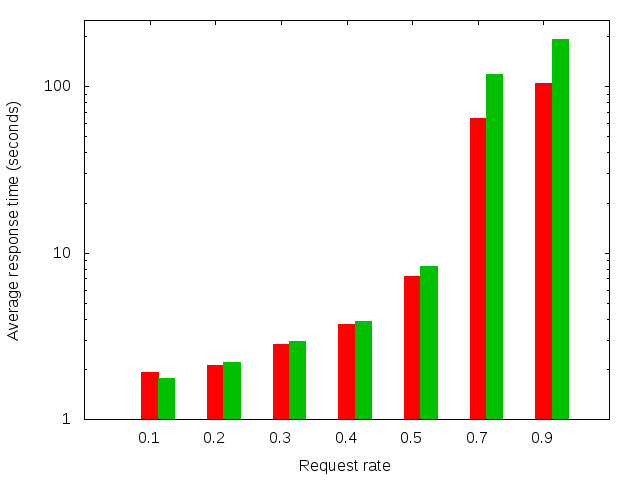
\includegraphics[width=0.5\linewidth]{responsetime_priority.png}
    \caption{Results with a priority queue (in red) vs results without (in green)}
    \label{fig:priorityqueue}
\end{figure}

\subsection{Measurements on a multi-threaded server}
\label{sub:Measurements on a multi-threaded server}

\subsubsection{Bottlenecks}
\label{subs:Bottlenecks}


\subsubsection{Multi-threading and queuing station model}
\label{subs:Multi-threading and queuing station model}
